\documentclass[9pt]{beamer}
\mode<presentation>

% Theme choice:
\usetheme{Madrid}%Darmstadt 

\usecolortheme[RGB={0,100,50}]{structure}
 \usefonttheme{structurebold} 
\setbeamercovered{invisible}
%\setbeamertemplate{navigation symbols}{}
\usepackage{dynblocks}
\usepackage{textpos}
\usepackage{amsfonts}
\usepackage{amsmath}
\usepackage{amssymb}
\usepackage{amsthm}

\newtheorem{teorema}{Teorema}\usepackage{mathtools}
\renewcommand{\proofname}{Prova}
\usepackage[portuguese]{babel}

\uselanguage{Portuguese}
\languagepath{Portuguese}

\deftranslation[to=Portuguese]{Theorem}{Teorema}
\deftranslation[to=Portuguese]{Lemma}{Lema}
\deftranslation[to=Portuguese]{Corollary}{Corolário}
\deftranslation[to=Portuguese]{Proof}{Prova}

\usepackage{dutchcal}
\usepackage{hyperref}
\usepackage[utf8]{inputenc}
\usepackage[T1]{fontenc}
\usepackage{amsthm}


\usepackage[affil-it]{authblk} 
\usepackage{etoolbox}
\usepackage{lmodern}

\makeatletter
\patchcmd{\@maketitle}{\LARGE \@title}{\fontsize{18}{19.2}\selectfont\@title}{}{}
\makeatother

\renewcommand\Authfont{\fontsize{12}{14.4}\selectfont}
\renewcommand\Affilfont{\fontsize{9}{10.8}\itshape}

% Title page details: 
\title[Presentation]{Lógica para Engenharia de Software} %add title


\institute[UniRV]{\textbf{\large  \textcolor{structure}{\textbf{\large
Uma introdução ao mundo das provas matemáticas: 
Axiomas, Definições, Teoremas, Lemas, Corolários.
}} %add name 
% \hspace{0.5pt}
\\ \qquad
\\Professor: Me. Sergio Souza Novak 
\\Faculdade de Engenharia de Software}
} 
% \titlegraphic{\includegraphics[width=5cm]{msu.eps}}
\titlegraphic{
\includegraphics[width=5cm]{Universidade_de_Rio_Verde.jpg}}
\date{}

% Logo only on title page
%\logo{
\includegraphics[width=1cm,keepaspectratio]{Logo.png}}
\usepackage[pscoord]{eso-pic}


\begin{document}

% Title page frame
%\begin{frame}
    %\titlepage 
%\end{frame}
\frame[plain]{\titlepage}
%logo
\AddToShipoutPictureFG{
    \put(\LenToUnit{.92\paperwidth},
    \LenToUnit{.185\paperheight})
    {\vtop{{\null}
    \makebox{
\includegraphics[width=.8cm,keepaspectratio]{Universidade_de_Rio_Verde.jpg}}}}}


\begin{frame}{Sumário}
  \tableofcontents
\end{frame}
\section{Introdução: Fermat e suas Provas}
% Slide 1: Introdução a Fermat
\begin{frame}{Pierre de Fermat (1607–1665)}
\begin{block}{Quem foi Fermat?}
Pierre de Fermat foi um matemático francês, advogado e funcionário público, conhecido por suas contribuições à teoria dos números, geometria analítica e cálculo de probabilidades.
\end{block}

\begin{itemize}
    \item Nascido em Beaumont-de-Lomagne, França.
    \item Estudou direito e trabalhou como magistrado.
    \item Matemático por paixão, escrevia suas descobertas em cartas e margens de livros.
\end{itemize}
\end{frame}

% Slide 2: Provas nas margens
\begin{frame}{Provas nas Margens dos Livros}
\begin{block}{Hábito curioso}
Fermat tinha o costume de escrever teoremas e esboços de provas nas margens dos livros que estudava, muitas vezes sem fornecer provas completas.
\end{block}

\begin{itemize}
    \item Seu estilo enigmático estimulou outros matemáticos a tentarem demonstrar suas conjecturas.
    \item A mais famosa é a ``Última Teorema de Fermat'', escrita na margem de um livro de Diofanto:
    \[
    x^n + y^n = z^n \quad \text{não possui soluções inteiras positivas para } n>2.
    \]
\end{itemize}
\end{frame}

% Slide 3: Histórico e legado
\begin{frame}{Histórico e Legado}
\begin{itemize}
    \item Muitas das provas de Fermat permaneciam incompletas ou apenas esboçadas.
    \item Suas ideias motivaram séculos de pesquisas em teoria dos números.
    \item A ``Última Teorema de Fermat'' foi provada somente em 1994 por Andrew Wiles, quase 350 anos depois.
    \item Contribuições importantes:
    \begin{itemize}
        \item Teorema de Fermat sobre somas de dois quadrados.
        \item Pequeno Teorema de Fermat.
        \item Fundamentos da teoria dos números e probabilidades.
    \end{itemize}
\end{itemize}
\end{frame}
\begin{frame}{Formalismo antigo matemático: Euclides, os elementos}
    \begin{figure}[H]
        \centering
        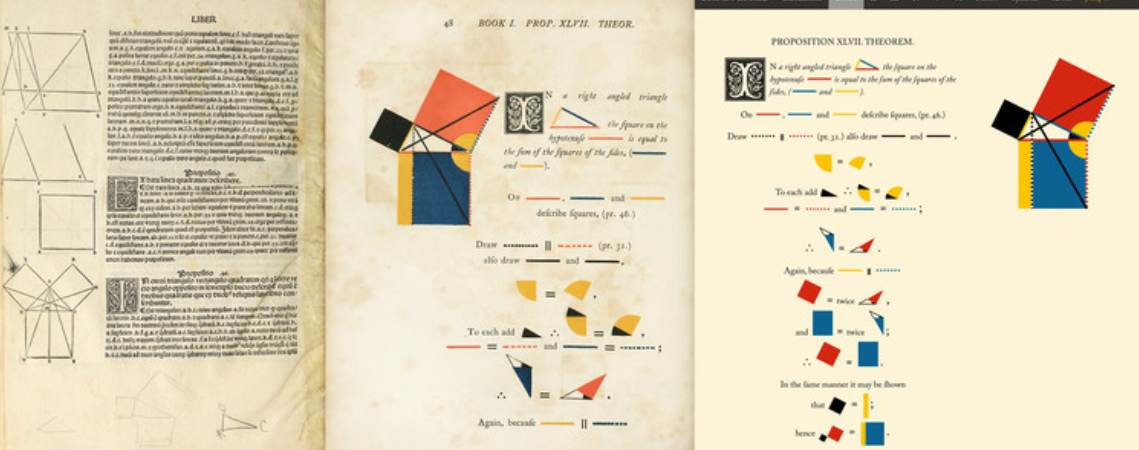
\includegraphics[width = 18cm]{euclides.png}
    \end{figure}
\end{frame}
\begin{frame}{Georg Cantor e o Formalismo Matemático}
\begin{block}{Quem foi Cantor?}
Georg Cantor (1845–1918) foi um matemático alemão, conhecido como o criador da \textbf{teoria dos conjuntos}, que revolucionou a forma de entender o infinito e a estrutura dos números.
\end{block}

\vspace{0.3cm}

\begin{block}{Principais Contribuições}
\begin{itemize}
    \item Introduziu a noção de \textbf{conjunto} como objeto matemático fundamental.
    \item Formalizou conceitos de \textbf{cardinalidade} e \textbf{ordinalidade} para comparar tamanhos de conjuntos.
    \item Distinguuiu diferentes tipos de \textbf{infinitos}, como \(\aleph_0\) (conjunto dos números naturais) e infinitos maiores.
    \item Desenvolveu o \textbf{diagonal argument} para provar que o conjunto dos números reais é não enumerável.
    \item Fundamentou o formalismo em matemática moderna, permitindo rigor na definição de números, funções e relações.
\end{itemize}
\end{block}

\end{frame}

\section{Axiomas}

\begin{frame}{Axioma}

\begin{block}{O que é}
Um axioma é uma proposição  básica aceita como \textbf{verdadeira sem demonstração}, usada como ponto de partida para construir uma teoria matemática ou lógica.
\end{block}
\pause

\begin{block}{Axioma da reta}
    "Dadas dois pontos distintos, existe uma única reta que os contém."
    \begin{figure}[H]
        \centering
        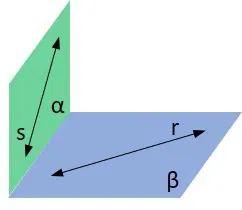
\includegraphics[width = 2cm]{retas.png}
    \end{figure}
    

\end{block}
    
\pause
\begin{block}{Axioma da escolha}
    "Dada uma coleção de conjuntos não vazios, é possível escolher um elemento de cada conjunto, mesmo que a coleção seja infinita."
\end{block}
\end{frame}
\begin{frame}
    \begin{block}{Axioma da escolha}
    "Dada uma coleção de conjuntos não vazios, é possível escolher um elemento de cada conjunto, mesmo que a coleção seja infinita."
\end{block}
\begin{block}{Axioma da escolha: Formalismo}

Dada uma família de conjuntos não vazios
\[
\{A_i\}_{i \in I},
\]
existe uma função de escolha
\[
f : I \to \bigcup_{i \in I} A_i
\]
tal que
\[
f(i) \in A_i \quad \text{para todo } i \in I.
\]
\end{block}
\end{frame}
% Slide 1: Existe
\begin{frame}{Quantificador Existencial — ``Existe''}

\begin{block}{Definição}
A expressão
\[
\exists x \in A,\; P(x)
\]
significa que existe \textbf{pelo menos um} elemento \(x\) no conjunto \(A\) para o qual a proposição \(P(x)\) é verdadeira.
\end{block}

\vspace{0.4cm}

\begin{block}{Leitura}
``Existe um \(x\) pertencente a \(A\) tal que \(P(x)\) é verdadeiro.''
\end{block}

\vspace{0.4cm}

\begin{block}{Exemplo}
\[
\exists n \in \mathbb{Z},\; n^2 = 4
\]
(A proposição é verdadeira para \(n = 2\) e \(n = -2\).)
\end{block}

\end{frame}

% Slide 2: Existe um único
\begin{frame}{Quantificador Existencial Único — ``Existe um único''}

\begin{block}{Definição}
A expressão
\[
\exists! x \in A,\; P(x)
\]
significa que existe \textbf{um e somente um} elemento \(x\) no conjunto \(A\) para o qual a proposição \(P(x)\) é verdadeira.
\end{block}

\vspace{0.4cm}

\begin{block}{Leitura}
``Existe um único \(x\) pertencente a \(A\) tal que \(P(x)\) é verdadeiro.''
\end{block}

\vspace{0.4cm}

\begin{block}{Exemplo}
\[
\exists! n \in \mathbb{N},\; n^2 = 1
\]
(A proposição é verdadeira apenas para \(n = 1\).)
\end{block}

\end{frame}

\section{Definições}

\begin{frame}{Definições}
    \begin{block}{O que é}
    Uma definição é uma proposição que estabelece \textbf{o significado de um termo ou conceito} dentro de uma teoria matemática ou lógica.
    \end{block}
    
    \pause
    
    \begin{block}{Definição de círculo}
    Um círculo é o conjunto de todos os pontos em um plano que estão a uma distância fixa, chamada de raio, de um ponto fixo, chamado de centro.
    \begin{figure}[H]
        \centering
        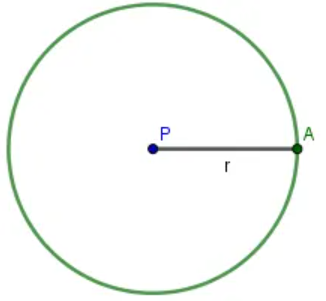
\includegraphics[width = 4cm]{circulo2.png}
    \end{figure}   
    \end{block}
\end{frame}
\begin{frame}{Explorando a definição de círculo }
 \begin{block}{Definição de círculo}
  
Sejam \( C = (a,b) \in \mathbb{R}^2 \) e \( r \in \mathbb{R} \), com \( r > 0 \).
O círculo de centro \( C \) e raio \( r \) é o conjunto
\[
\mathcal{C}(C,r) = \{ (x,y) \in \mathbb{R}^2 \mid (x-a)^2 + (y-b)^2 = r^2 \}.
\]
\end{block}

\end{frame}

\begin{frame}{Aplicando a definição de círculo }

Considere o círculo de centro \( C = (0,0) \) e raio \( r = 5 \).

Verifique se os pontos abaixo pertencem ao círculo:
\[
P_1 = (3,4), \quad P_2 = (5,0), \quad P_3 = (2,2).
\]

\textbf{Critério:}  
Calcule \( x^2 + y^2 \) e compare com \( r^2 = 25 \).

\begin{itemize}
\item Se \( x^2 + y^2 = 25 \), o ponto pertence ao círculo.
\item Se \( x^2 + y^2 < 25 \), o ponto está no disco.
\item Se \( x^2 + y^2 > 25 \), o ponto está fora.
\end{itemize}
    \pause


O círculo tem centro \( C = (0,0) \) e raio \( r = 5 \), logo \( r^2 = 25 \).

\begin{itemize}
\item \textbf{Ponto \( P_1 = (3,4) \):}
\[
3^2 + 4^2 = 9 + 16 = 25.
\]
Como \( x^2 + y^2 = 25 \), o ponto \( P_1 \) pertence ao círculo.

\item \textbf{Ponto \( P_2 = (5,0) \):}
\[
5^2 + 0^2 = 25.
\]
Como \( x^2 + y^2 = 25 \), o ponto \( P_2 \) pertence ao círculo.

\item \textbf{Ponto \( P_3 = (2,2) \):}
\[
2^2 + 2^2 = 4 + 4 = 8.
\]
Como \( x^2 + y^2 < 25 \), o ponto \( P_3 \) não pertence ao círculo; ele está no interior do disco.
\end{itemize}

\end{frame}

\begin{frame}{Melhor e pior caso de um Algoritmo}
    \begin{block}{O que é}
    O melhor e o pior caso de um algoritmo referem-se às análises de desempenho em termos de tempo de execução ou uso de recursos, considerando as entradas mais favoráveis (melhor caso) e as mais desfavoráveis (pior caso).
    \end{block}
       \begin{figure}
        \centering
        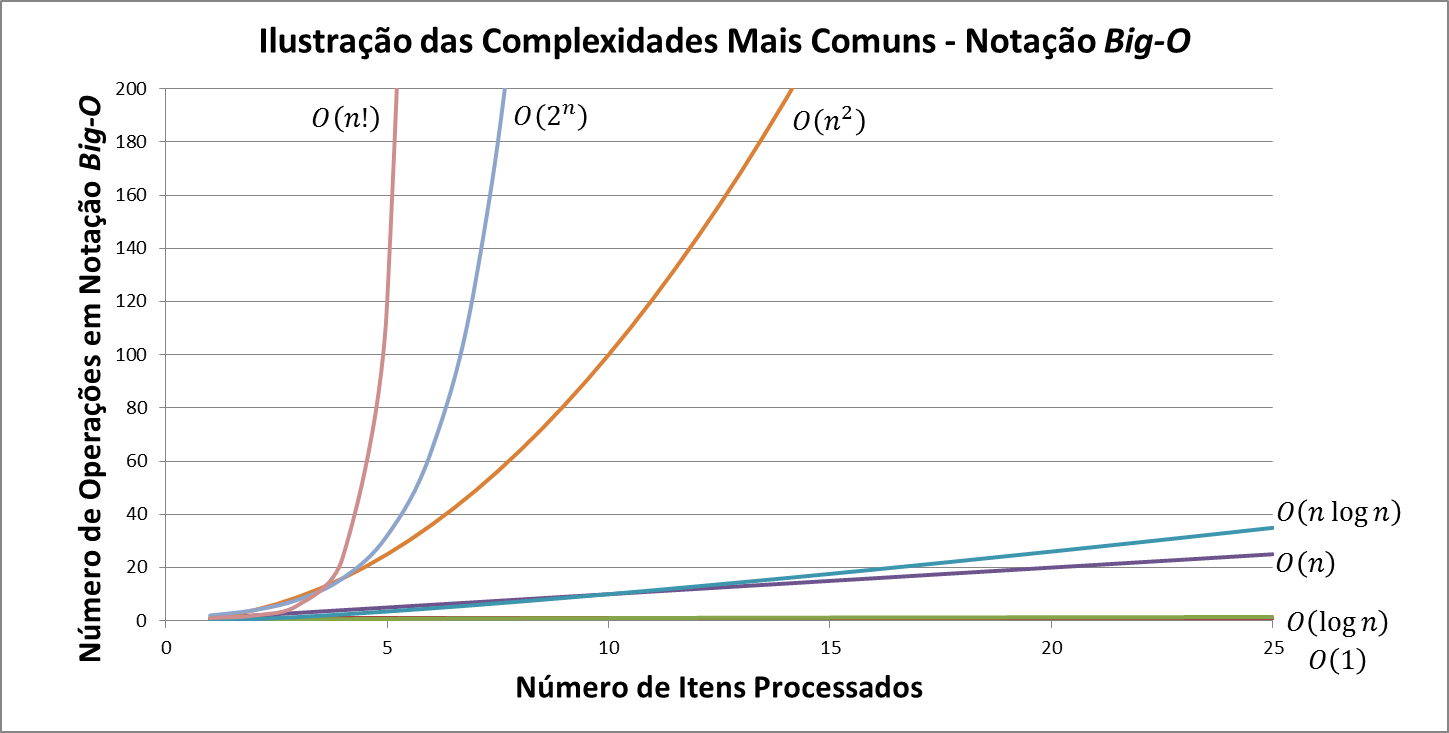
\includegraphics[width = 9cm]{BigOGraph.png}
    \end{figure}
    \end{frame}
\begin{frame}{Melhor e pior caso de um Algoritmo}

    \begin{block}{O que é}
    O melhor e o pior caso de um algoritmo referem-se às análises de desempenho em termos de tempo de execução ou uso de recursos, considerando as entradas mais favoráveis (melhor caso) e as mais desfavoráveis (pior caso).
    \end{block}
    \begin{block}{Exemplo: Busca Linear}
    Considere um algoritmo de busca linear que procura um elemento em uma lista não ordenada.
    \begin{itemize}
        \item \textbf{Melhor Caso:} O elemento está na primeira posição da lista. O algoritmo encontra o elemento imediatamente, resultando em um tempo de execução constante \( O(1) \).
        \item \textbf{Pior Caso:} O elemento está na última posição da lista ou não está presente. O algoritmo precisa verificar todos os elementos, resultando em um tempo de execução linear \( O(n) \), onde \( n \) é o número de elementos na lista.
    \end{itemize}
    \end{block}
\end{frame}
\begin{frame}{Melhor e pior caso de um Algoritmo}

\begin{block}{Casos de execução}
Seja \( T(I) \) o tempo de execução de um algoritmo para uma entrada \( I \) de tamanho \( |I| = n \).

\begin{itemize}
\item \textbf{Pior caso (worst case):}  
Define-se o tempo de execução no pior caso como
\[
T_{\text{pior}}(n) = \max \{ T(I) \mid |I| = n \}.
\]

\item \textbf{Melhor caso (best case):}  
Define-se o tempo de execução no melhor caso como
\[
T_{\text{melhor}}(n) = \min \{ T(I) \mid |I| = n \}.
\]

\item \textbf{Caso médio (average case):}  
Seja \( \mathcal{I}_n \) o conjunto de todas as entradas de tamanho \( n \) e
\( p : \mathcal{I}_n \to [0,1] \) uma distribuição de probabilidade sobre \( \mathcal{I}_n \).
Define-se o tempo de execução no caso médio como
\[
T_{\text{médio}}(n) = \sum_{I \in \mathcal{I}_n} T(I)\, p(I).
\]
\end{itemize}
\end{block}
\end{frame}
\section{Lemas}

\begin{frame}{Quantificador Universal — ``Para todo''}

\begin{block}{Definição}
A expressão
\[
\forall x \in A,\; P(x)
\]
significa que a proposição \(P(x)\) é verdadeira para \textbf{todos} os elementos
\(x\) do conjunto \(A\).
\end{block}

\vspace{0.4cm}

\begin{block}{Leitura}
``Para todo \(x\) pertencente a \(A\), vale \(P(x)\).''
\end{block}

\vspace{0.4cm}

\begin{block}{Definição (Conjunto Vazio)}
Um conjunto \( A \) é chamado de \textbf{conjunto vazio} se, e somente se,
\[
\forall x,\; x \notin A.
\]
Denotamos o conjunto vazio por \( \varnothing \).
\end{block}

\end{frame}





\begin{frame}{Teorema}
\begin{block}{O que é um teorema?}


Um \emph{teorema} é uma proposição matemática
cuja veracidade é demonstrada de forma rigorosa
a partir de axiomas, definições e resultados previamente estabelecidos.
    \end{block}

\vspace{0.4cm}

\textbf{Características principais}

\begin{itemize}
\item Possui um enunciado preciso e bem definido;
\item Exige uma demonstração formal;
\item Representa um resultado central dentro de uma teoria.
\end{itemize}

\end{frame}
\begin{frame}{Definição de Número Par}

\begin{block}{Definição}
Um número inteiro \( n \in \mathbb{Z} \) é chamado de \textbf{par} se existe
um inteiro \( k \in \mathbb{Z} \) tal que
\[
n = 2k.
\]
\end{block}

\vspace{0.4cm}

\begin{block}{Observações}
\begin{itemize}
\item A definição é \textbf{existencial}: basta a existência de um inteiro \(k\);
\item Todo número par é múltiplo de \(2\);
\item A paridade é uma propriedade fundamental em provas matemáticas.
\end{itemize}
\end{block}

\vspace{0.4cm}

\begin{block}{Exemplos}
\[
-4 = 2(-2), \quad 0 = 2(0), \quad 8 = 2(4)
\]
\end{block}

\end{frame}

\begin{frame}{Teorema Clássico — Números Pares}

\begin{theorem}[Soma de números pares]
Se \(a\) e \(b\) são números inteiros pares, então \(a + b\) também é um número par.
\end{theorem}

\begin{proof}
Como \(a\) e \(b\) são pares, existem inteiros \(k\) e \(m\) tais que
\[
a = 2k \quad \text{e} \quad b = 2m.
\]
Logo,
\[
a + b = 2k + 2m = 2(k+m),
\]
onde \(k+m\) é um inteiro. Portanto, \(a + b\) é par.
\end{proof}

\end{frame}
\begin{frame}{Exercícios — Provas com Números Pares}

\begin{block}{Exercício 1}
Prove que a soma de dois números inteiros ímpares é um número par.
\end{block}

\begin{block}{Dica}
Use a definição formal de número ímpar:
\[
n \in \mathbb{Z} \text{ é ímpar } \iff \exists k \in \mathbb{Z}
\text{ tal que } n = 2k + 1.
\]
\end{block}
\vspace{0.3cm}

\begin{block}{Exercício 2}
Prove que o produto de um número inteiro par por qualquer número inteiro é par.
\end{block}

\vspace{0.3cm}

\begin{block}{Exercício 3}
Mostre que, se \( n \) é um inteiro par, então \( n^2 \) também é par.
\end{block}

\vspace{0.3cm}


\end{frame}
\begin{frame}{Respostas — Provas com Números Pares}

\begin{block}{Resposta do Exercício 1}
Sejam \(a,b \in \mathbb{Z}\) números ímpares.  
Então existem \(k,m \in \mathbb{Z}\) tais que
\[
a = 2k+1 \quad \text{e} \quad b = 2m+1.
\]
Logo,
\[
a+b = (2k+1)+(2m+1) = 2(k+m+1),
\]
que é um número par.
\end{block}

\vspace{0.3cm}

\begin{block}{Resposta do Exercício 2}
Seja \(a \in \mathbb{Z}\) um número par.  
Então existe \(k \in \mathbb{Z}\) tal que \(a = 2k\).
Para qualquer \(b \in \mathbb{Z}\),
\[
a\cdot b = (2k)b = 2(kb),
\]
logo o produto é par.
\end{block}

\vspace{0.3cm}
\end{frame}
\begin{frame}{Respostas — Provas com Números Pares}
\begin{block}{Resposta do Exercício 3}
Se \(n \in \mathbb{Z}\) é par, então existe \(k \in \mathbb{Z}\) tal que
\[
n = 2k.
\]
Assim,
\[
n^2 = (2k)^2 = 4k^2 = 2(2k^2),
\]
o que mostra que \(n^2\) é par. 
\end{block}

\end{frame}

\begin{frame}{Lema}

\textbf{O que é um lema?}

Um \emph{lema} é um resultado matemático demonstrável
utilizado como \textbf{passo auxiliar} na prova de um teorema.

\vspace{0.4cm}

\textbf{Função do lema}

\begin{itemize}
\item Simplificar provas longas ou complexas;
\item Isolar argumentos técnicos importantes;
\item Evitar repetição de ideias em demonstrações.
\end{itemize}

\vspace{0.4cm}

\textbf{Relação com outros resultados}

\begin{itemize}
\item Um lema tem o mesmo valor lógico que um teorema;
\item A diferença está no \textbf{papel didático}, não na validade;
\item Lemas podem originar teoremas ou corolários.
\end{itemize}

\vspace{0.4cm}

\textbf{Exemplo}

\begin{itemize}
\item \textbf{Lema:} No pior caso, a busca linear realiza \( n \) comparações.
\item \textbf{Teorema:} A busca linear tem complexidade \( \Theta(n) \).
\end{itemize}

\end{frame}

\section{Corolários}
\begin{frame}{Corolário}
    \begin{block}{O que é}
Um corolário é um resultado que decorre \textbf{imediatamente}
de um teorema ou lema já demonstrado, sem necessidade de uma nova prova elaborada.
    \end{block}


\textbf{Definição}

Um enunciado é chamado de \emph{corolário} quando sua validade
segue diretamente de um resultado anterior.

\vspace{0.4cm}

\textbf{Exemplo}

\begin{itemize}
\item \textbf{Lema:} Se \( f(n) = an + b \), com \( a > 0 \), então
\( f(n) \in \Theta(n) \).
\item \textbf{Corolário:} Todo algoritmo com tempo de execução linear
possui complexidade \( \Theta(n) \).
\end{itemize}

\vspace{0.4cm}

\textbf{Observação}

Normalmente, a prova de um corolário é curta ou indicada pela frase:
``Segue diretamente do resultado anterior.''

\end{frame}
\begin{frame}{Corolário — Busca Linear}

\textbf{Contexto}

Considere o algoritmo de \emph{busca linear} aplicado a um vetor
com \( n \) elementos.

\vspace{0.4cm}

\textbf{Lema (anterior)}

No pior caso, a busca linear realiza \( n \) comparações.

\vspace{0.4cm}

\textbf{Corolário}

O algoritmo de busca linear possui complexidade de tempo
\[
\Theta(n)
\]
no pior caso.

\vspace{0.4cm}

\textbf{Justificativa}

O resultado segue diretamente do fato de que o número de comparações
cresce linearmente com o tamanho da entrada.

\end{frame}
\begin{frame}{Teorema e Corolário}


O corolário é um teorema?
    \pause

\vspace{0.4cm}

\textbf{Resposta}

Sim. Um \emph{corolário} é um tipo particular de \emph{teorema}.

\vspace{0.4cm}

\textbf{Diferença conceitual}

\begin{itemize}
\item \textbf{Teorema:} resultado principal, de maior relevância conceitual,
que exige uma demonstração completa.
\item \textbf{Corolário:} resultado que decorre diretamente de um teorema
ou lema anterior, com demonstração imediata ou trivial.
\end{itemize}

\vspace{0.4cm}
    \pause

\begin{block}{Interpretação didática}


Todo corolário é um teorema, mas nem todo teorema é um corolário.
A distinção é didática e organizacional, não lógica.

\end{block}



\end{frame}


\begin{frame}{Exercícios — Provas com Números Racionais}

Use a definição formal:
\[
x \in \mathbb{Q} \iff \exists a,b \in \mathbb{Z},\ b \neq 0
\text{ tais que } x = \frac{a}{b}.
\]
\begin{block}{Exercício 1}
Prove que a soma de dois números racionais é um número racional.
\end{block}


\begin{block}{Exercício 2}
Prove que o produto de um número racional por um número inteiro é racional.
\end{block}


\begin{block}{Exercício 3}
Mostre que o quadrado de um número racional é um número racional.
\end{block}


\begin{block}{Exercício 4}
Prove que a diferença entre dois números racionais é um número racional.
\end{block}




\end{frame}

\begin{frame}{Exercícios — Respostas com Números Racionais}

\begin{block}{Exercício 1 — Soma de racionais}
Sejam \(x = \frac{a}{b}\) e \(y = \frac{c}{d}\) dois números racionais, com \(a,b,c,d \in \mathbb{Z}\) e \(b,d \neq 0\).  
Então,
\[
x + y = \frac{a}{b} + \frac{c}{d} = \frac{ad + bc}{bd}.
\]  
Como \(ad + bc \in \mathbb{Z}\) e \(bd \neq 0\), segue que \(x + y \in \mathbb{Q}\).
\end{block}

\vspace{0.3cm}

\begin{block}{Exercício 2 — Produto com inteiro}
Seja \(x = \frac{a}{b} \in \mathbb{Q}\) e \(k \in \mathbb{Z}\).  
Então,
\[
k \cdot x = k \cdot \frac{a}{b} = \frac{ka}{b}.
\]  
Como \(ka \in \mathbb{Z}\) e \(b \neq 0\), temos \(k \cdot x \in \mathbb{Q}\).
\end{block}

\vspace{0.3cm}
\end{frame}
\begin{frame}{Exercícios — Respostas com Números Racionais}
\begin{block}{Exercício 3 — Quadrado de um racional}
Seja \(x = \frac{a}{b} \in \mathbb{Q}\).  
Então,
\[
x^2 = \left(\frac{a}{b}\right)^2 = \frac{a^2}{b^2}.
\]  
Como \(a^2, b^2 \in \mathbb{Z}\) e \(b^2 \neq 0\), segue que \(x^2 \in \mathbb{Q}\).
\end{block}

\vspace{0.3cm}

\begin{block}{Exercício 4 — Diferença de racionais}
Sejam \(x = \frac{a}{b}\) e \(y = \frac{c}{d}\) dois números racionais.  
Então,
\[
x - y = \frac{a}{b} - \frac{c}{d} = \frac{ad - bc}{bd}.
\]  
Como \(ad - bc \in \mathbb{Z}\) e \(bd \neq 0\), segue que \(x - y \in \mathbb{Q}\).
\end{block}

\end{frame}



\begin{frame}{Bons estudos!}
    \begin{figure}
        \centering
        
\includegraphics[width = 9cm]{Universidade_de_Rio_Verde.jpg}
    \end{figure}
\end{frame}





\end{document}
